\documentclass[border=5pt]{standalone}
\usepackage{tikz}
\usepackage{xcolor}
\usetikzlibrary{positioning, calc}

\begin{document}

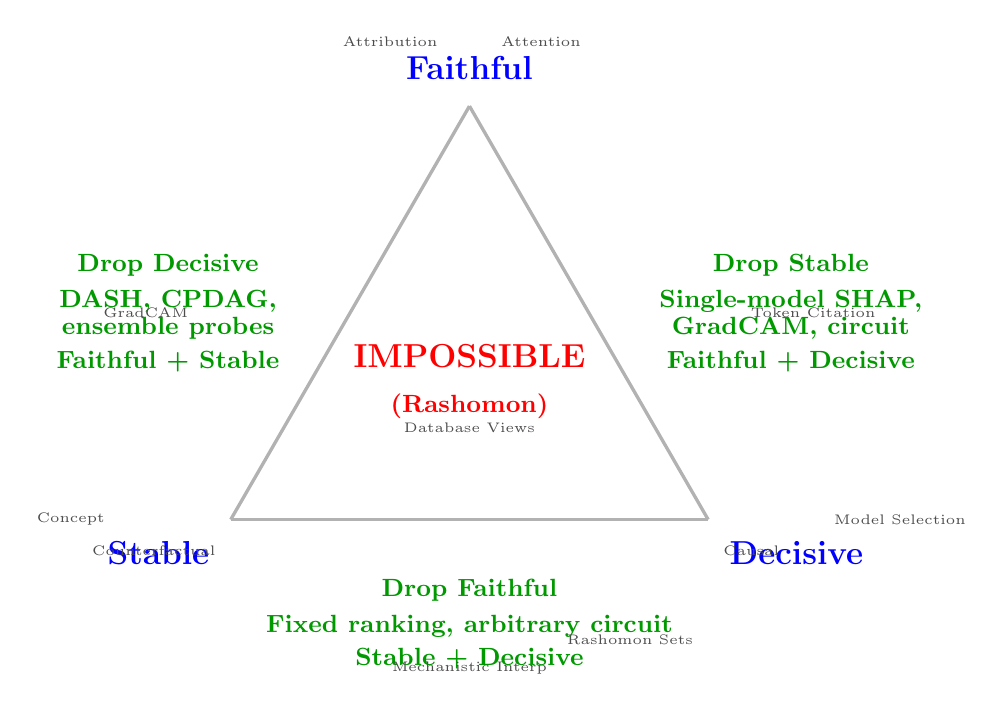
\begin{tikzpicture}[
  vertex/.style={font=\large\bfseries, text=blue},
  impossible/.style={font=\large\bfseries, text=red, align=center},
  edgelabel/.style={font=\small\bfseries, text=green!60!black, align=center},
  edgesub/.style={font=\footnotesize, text=green!50!black, align=center},
  instance/.style={font=\tiny, text=black!70, align=center},
  scale=3.5
]

%% Triangle vertices (equilateral, centered at origin)
\coordinate (Faithful) at (0, 1);
\coordinate (Stable)   at ({-sqrt(3)/2}, -0.5);
\coordinate (Decisive) at ({sqrt(3)/2},  -0.5);

%% Draw triangle edges
\draw[thick, gray!60, line width=1.2pt] (Faithful) -- (Stable);
\draw[thick, gray!60, line width=1.2pt] (Faithful) -- (Decisive);
\draw[thick, gray!60, line width=1.2pt] (Stable)   -- (Decisive);

%% Vertex labels (blue, outside the triangle)
\node[vertex, above=6pt] at (Faithful) {Faithful};
\node[vertex, below left=6pt] at (Stable) {Stable};
\node[vertex, below right=6pt] at (Decisive) {Decisive};

%% Center: IMPOSSIBLE
\node[impossible] at (0, 0) {IMPOSSIBLE\\[2pt]{\small (Rashomon)}};

%% -------------------------------------------------------
%% EDGE LABELS
%% -------------------------------------------------------

%% Bottom edge: Stable -- Decisive  (Drop Faithful)
%% Midpoint of bottom edge is at (0, -0.5)
\node[edgelabel, below=18pt] at ($(Stable)!0.5!(Decisive)$)
  {Drop Faithful\\[2pt]
   {\small Fixed ranking, arbitrary circuit}\\[1pt]
   \edgesub{Stable + Decisive}};

%% Left edge: Faithful -- Stable  (Drop Decisive)
%% Midpoint of left edge
\node[edgelabel, left=22pt] at ($(Faithful)!0.5!(Stable)$)
  {Drop Decisive\\[2pt]
   {\small DASH, CPDAG,}\\[-1pt]
   {\small ensemble probes}\\[1pt]
   \edgesub{Faithful + Stable}};

%% Right edge: Faithful -- Decisive  (Drop Stable)
%% Midpoint of right edge
\node[edgelabel, right=22pt] at ($(Faithful)!0.5!(Decisive)$)
  {Drop Stable\\[2pt]
   {\small Single-model SHAP,}\\[-1pt]
   {\small GradCAM, circuit}\\[1pt]
   \edgesub{Faithful + Decisive}};

%% -------------------------------------------------------
%% 9 INSTANCE LABELS around the outside of the triangle
%% -------------------------------------------------------

%% Near Faithful vertex (top): Attribution, Attention
\node[instance, above left=18pt and 8pt] at (Faithful)
  {Attribution};
\node[instance, above right=18pt and 8pt] at (Faithful)
  {Attention};

%% Near Stable vertex (bottom-left): Counterfactual, Concept
\node[instance, below left=6pt and 2pt] at (Stable)
  {Counterfactual};
\node[instance, left=42pt] at (Stable)
  {Concept};

%% Near Decisive vertex (bottom-right): Causal, Model Selection
\node[instance, below right=6pt and 2pt] at (Decisive)
  {Causal};
\node[instance, right=42pt] at (Decisive)
  {Model Selection};

%% Along left edge (between Faithful and Stable): GradCAM
\node[instance, left=55pt] at ($(Faithful)!0.5!(Stable)$)
  {GradCAM};

%% Along right edge (between Faithful and Decisive): Token Citation
\node[instance, right=55pt] at ($(Faithful)!0.5!(Decisive)$)
  {Token Citation};

%% Additional Tier 1 instances: Database, Statistics
\node[instance, above=28pt] at ($(Stable)!0.5!(Decisive)$)
  {Database Views};
\node[instance, below left=38pt and 2pt] at (Decisive)
  {Rashomon Sets};

%% Along bottom edge (between Stable and Decisive): Mechanistic Interp
\node[instance, below=48pt] at ($(Stable)!0.5!(Decisive)$)
  {Mechanistic Interp};

\end{tikzpicture}

\end{document}
